\documentclass[a4paper,10pt]{article}


% <<<<<<<<<<<<<<<<<
%  PACKAGE IMPORTS
% <<<<<<<<<<<<<<<<<

% Required
\usepackage[margin=2.54cm, headheight=10pt]{geometry}
\usepackage{hyperref}
\usepackage{parskip}
\usepackage{graphicx}
\usepackage{float}
\usepackage{xcolor}
\usepackage{setspace}
\usepackage{amsfonts}
\usepackage{amsmath} 
\usepackage{amssymb}
\usepackage{mathrsfs}
\usepackage[normalem]{ulem}
\usepackage{fancyvrb}
\usepackage{mathrsfs}
\usepackage{pgfplots}
\usepackage{tocloft}
\usepackage{fancyhdr}

% Optional
\usepackage[breakable]{tcolorbox}
\usepackage{mdframed}

% Temporary
\usepackage{blindtext}



% <<<<<<<<<<<<<<<<<
%  PACKAGE SETTINGS
% <<<<<<<<<<<<<<<<<

\definecolor{urlcolor}{rgb}{0,.145,.698}
\definecolor{linkcolor}{rgb}{.15,.15,.15}
\definecolor{citecolor}{rgb}{.12,.54,.11}


% Define a nice break command that doesn't care if a line doesn't already exist.
\def\br{\hspace*{\fill} \\* }

\sloppy
\hypersetup{
  breaklinks=true,  % so long urls are correctly broken across lines
  colorlinks=true,
  urlcolor=urlcolor,
  linkcolor=linkcolor,
  citecolor=citecolor,
}

% TOC/LOF/LOT setup for a *short* table
\renewcommand{\cftsecdotsep}{\cftdotsep}
\renewcommand\cftaftertoctitle{\vspace{-0.3cm}\par\noindent\hrulefill\par\vspace{-0.4cm}}
\setlength{\cftsecindent}{0.8cm}
\setlength{\cftsubsecindent}{2cm}
\setlength{\cftsubsubsecindent}{3cm}
\setlength{\cftbeforesecskip}{0.25cm}

\renewcommand{\baselinestretch}{1.05}

% Fonts used
\usepackage{lmodern}




% <<<<<<<<<<<<<<<<<
%      DOCUMENT
% <<<<<<<<<<<<<<<<<

\title{\scshape Document Title}
\author{\bfseries Anton Slavin}
\date{\today}


\begin{document}

% Custom header and footer settings
\pagestyle{fancy}
\fancyhf{}
\renewcommand{\headrulewidth}{0pt}
%\fancyhead[LE]{\small \scshape \nouppercase{\thepage\hfill\leftmark}}
%\fancyhead[RO]{\small \scshape \nouppercase{\leftmark\hfill\thepage}}
\fancyfoot[LE,RO]{\hfill\thepage\hfill}



\maketitle
\vspace{0.5cm}
\tableofcontents
\vspace{-0.4cm}
\noindent\hrulefill

\vspace{0.5cm}

% \input for in-place, otherwise \chapter
\blinddocument

\blindtext[1]

\begin{figure}[H]
\centering
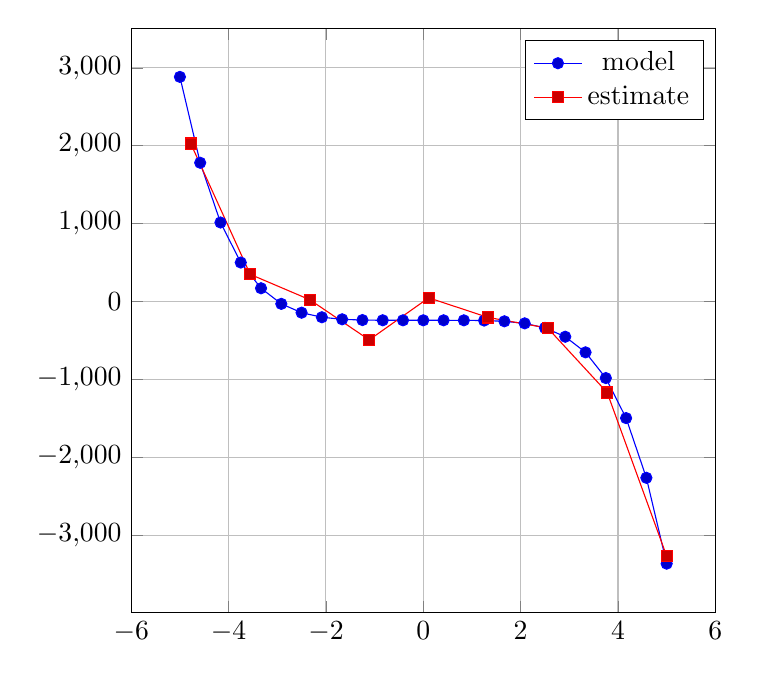
\begin{tikzpicture}
	\begin{axis}[
		height=9cm,
		width=9cm,
		grid=major,
	]
		
	\addplot {-x^5 - 242};
	\addlegendentry{model}

	\addplot coordinates {
		(-4.77778,2027.60977)
		(-3.55556,347.84069)
		(-2.33333,22.58953)
		(-1.11111,-493.50066)
		(0.11111,46.66082)
		(1.33333,-205.56286)
		(2.55556,-341.40638)
		(3.77778,-1169.24780)
		(5.00000,-3269.56775)
	};
	\addlegendentry{estimate}
	\end{axis}
\end{tikzpicture}
\caption{Some figure from \url{https://pgfplots.sourceforge.net/gallery.html}}
\end{figure}

\blindtext[1] 
\section{Section 2}

\blindmathpaper


\end{document}


